%==============================================================================
% Chapitre 50 - Les munitions militaires
%==============================================================================

\section{Introduction}

Depuis l'apparition des armes à feu modernes, les besoins militaires ont
fortement influencé le développement des munitions.

Les conflits armés ont conduit à la création de nombreuses cartouches devenues
par la suite des références dans le domaine civil.

Aujourd'hui encore, les exigences militaires constituent un moteur important
de l'innovation balistique.

\begin{aretenir}

De nombreuses cartouches civiles modernes trouvent leur origine dans des
munitions développées pour un usage militaire.

\end{aretenir}

\section{Objectifs militaires}

Une munition militaire doit répondre à plusieurs exigences parfois
contradictoires :

\begin{itemize}
    \item efficacité ;
    \item fiabilité ;
    \item robustesse ;
    \item coût maîtrisé ;
    \item facilité de production ;
    \item compatibilité logistique.
\end{itemize}

Ces contraintes influencent fortement sa conception.

\section{Standardisation}

Les armées utilisent généralement des munitions standardisées.

Cette standardisation facilite :

\begin{itemize}
    \item la fabrication ;
    \item le stockage ;
    \item le transport ;
    \item l'interopérabilité entre unités.
\end{itemize}

Elle constitue un élément essentiel de la logistique militaire.

\section{Le rôle de l'OTAN}

Au sein de l'OTAN, plusieurs cartouches ont été normalisées afin de permettre
leur emploi par différents pays.

Parmi les plus connues figurent :

\begin{itemize}
    \item le 5,56×45 mm ;
    \item le 7,62×51 mm ;
    \item le 9×19 mm.
\end{itemize}

Ces munitions sont utilisées par de nombreuses forces armées.

\section{La fiabilité avant tout}

Une munition militaire doit fonctionner dans des conditions difficiles :

\begin{itemize}
    \item températures extrêmes ;
    \item humidité ;
    \item poussière ;
    \item vibrations ;
    \item stockage prolongé.
\end{itemize}

La fiabilité constitue souvent le critère prioritaire.

\section{Production à grande échelle}

Les besoins militaires peuvent atteindre plusieurs millions de cartouches.

Les procédés industriels doivent donc permettre :

\begin{itemize}
    \item une cadence élevée ;
    \item une qualité constante ;
    \item un coût raisonnable.
\end{itemize}

\section{Munitions d'arme de poing}

Les armes de poing militaires utilisent généralement des cartouches offrant :

\begin{itemize}
    \item un recul modéré ;
    \item une bonne fiabilité ;
    \item un encombrement réduit.
\end{itemize}

Le 9×19 mm constitue aujourd'hui l'exemple le plus répandu.

\section{Munitions de fusil}

Les fusils militaires utilisent des cartouches adaptées aux engagements à
moyenne distance.

Leurs caractéristiques doivent permettre :

\begin{itemize}
    \item une portée suffisante ;
    \item une trajectoire acceptable ;
    \item une masse raisonnable.
\end{itemize}

\section{Évolution historique}

Durant le XX\ieme\ siècle, plusieurs tendances majeures sont apparues :

\begin{itemize}
    \item réduction du calibre ;
    \item augmentation de la vitesse ;
    \item allègement de la munition ;
    \item amélioration de la portée utile.
\end{itemize}

\begin{figure}[htbp]
\centering

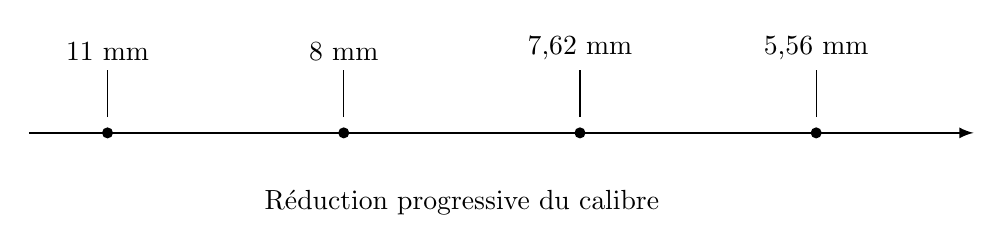
\begin{tikzpicture}[scale=1]

% Ligne principale
\draw[-latex,thick] (0,0) -- (12,0);

% Jalons
\foreach \x/\txt in {
1/{11 mm},
4/{8 mm},
7/{7,62 mm},
10/{5,56 mm}
}
{
    \fill (\x,0) circle (2pt);
    \draw (\x,0.2) -- (\x,0.8);
    \node[above] at (\x,0.8) {\txt};
}

\node[below] at (5.5,-0.6)
{Réduction progressive du calibre};

\end{tikzpicture}

\caption{Évolution simplifiée de certains calibres militaires au cours du temps.}
\label{fig:evolution_calibres_militaires}

\end{figure}

\section{Du calibre intermédiaire}

Après la Seconde Guerre mondiale, plusieurs armées ont adopté le concept de
cartouche intermédiaire.

Cette approche vise à trouver un compromis entre :

\begin{itemize}
    \item puissance ;
    \item portée ;
    \item contrôle du recul ;
    \item quantité de munitions transportées.
\end{itemize}

\begin{figure}[htbp]
\centering

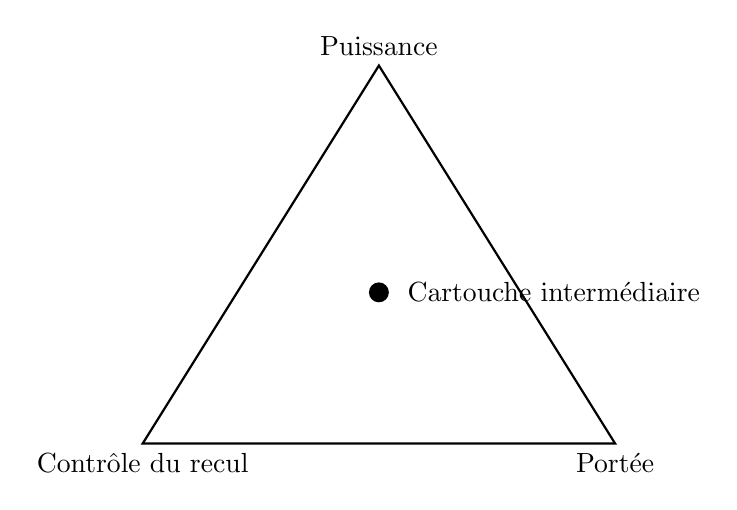
\begin{tikzpicture}[scale=1.2]

% Triangle
\draw[thick]
(0,0)
--
(5,0)
--
(2.5,4)
--
cycle;

% Sommets
\node[below] at (0,0)
{Contrôle du recul};

\node[below] at (5,0)
{Portée};

\node[above] at (2.5,4)
{Puissance};

% Point central
\fill (2.5,1.6) circle (3pt);

\node[right] at (2.7,1.6)
{Cartouche intermédiaire};

\end{tikzpicture}

\caption{Le calibre intermédiaire constitue un compromis entre plusieurs exigences contradictoires.}
\label{fig:calibre_intermediaire}

\end{figure}

\section{Exemple du 5,56×45 mm}

Le 5,56×45 mm est conçu pour offrir :

\begin{itemize}
    \item une vitesse élevée ;
    \item une masse réduite ;
    \item un recul limité ;
    \item une bonne capacité d'emport.
\end{itemize}

Son adoption a profondément influencé les armes militaires modernes.

\section{Exemple du 7,62×51 mm}

Le 7,62×51 mm conserve :

\begin{itemize}
    \item une énergie importante ;
    \item une portée significative ;
    \item une bonne capacité de pénétration.
\end{itemize}

Il reste largement utilisé dans certaines fonctions spécialisées.

\section{Munitions de mitrailleuse}

Les mitrailleuses utilisent souvent les mêmes cartouches que les fusils ou des
versions plus puissantes.

Les contraintes principales concernent :

\begin{itemize}
    \item l'échauffement ;
    \item la cadence de tir ;
    \item l'alimentation continue.
\end{itemize}

\section{Les munitions traçantes}

Les projectiles traçants produisent une trace lumineuse visible pendant le vol.

Ils permettent notamment :

\begin{itemize}
    \item l'observation de la trajectoire ;
    \item le réglage du tir ;
    \item la désignation d'objectif.
\end{itemize}

\section{Les munitions perforantes}

Certaines munitions sont conçues pour améliorer la pénétration.

Elles utilisent souvent un noyau réalisé dans un matériau plus dur que le
plomb.

\section{Les munitions incendiaires}

Les munitions incendiaires embarquent une composition capable de produire un
effet thermique important après impact.

\section{Les munitions d'exercice}

Les forces armées utilisent également :

\begin{itemize}
    \item des munitions d'entraînement ;
    \item des munitions à blanc ;
    \item des cartouches d'exercice inertes.
\end{itemize}

Ces munitions réduisent les coûts et améliorent la sécurité.

\begin{figure}[htbp]
\centering

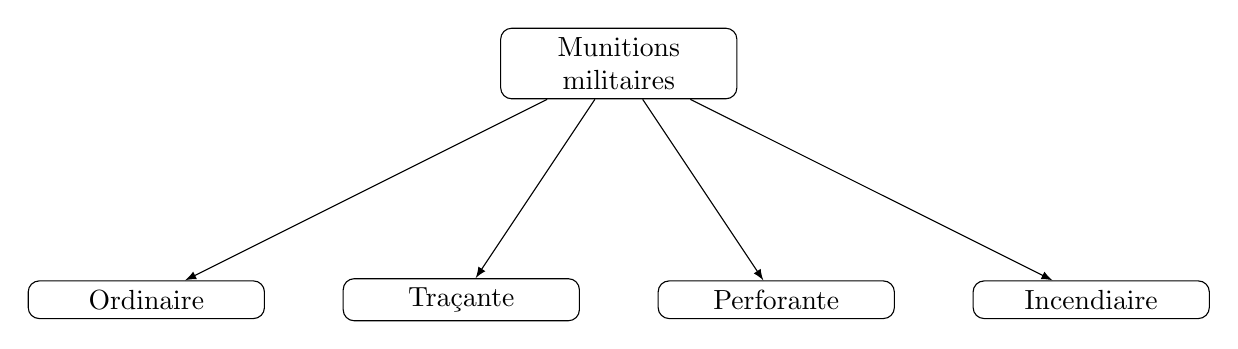
\begin{tikzpicture}[
every node/.style={
draw,
rounded corners,
align=center,
minimum width=3cm
}
]

\node (M) at (0,0) {Munitions\\militaires};

\node (B) at (-6,-3) {Ordinaire};
\node (T) at (-2,-3) {Traçante};
\node (P) at (2,-3) {Perforante};
\node (I) at (6,-3) {Incendiaire};

\draw[-latex] (M) -- (B);
\draw[-latex] (M) -- (T);
\draw[-latex] (M) -- (P);
\draw[-latex] (M) -- (I);

\end{tikzpicture}

\caption{Exemples de familles de munitions militaires spécialisées.}
\label{fig:types_munitions_militaires}

\end{figure}

\section{Stockage militaire}

Le stockage constitue un aspect essentiel de la logistique.

Les munitions doivent conserver leurs performances pendant de nombreuses
années.

Des procédures strictes encadrent :

\begin{itemize}
    \item le transport ;
    \item le stockage ;
    \item la surveillance des lots.
\end{itemize}

\section{Vers les projectiles militaires}

Les contraintes militaires ont conduit au développement de nombreux types de
projectiles spécialisés.

Le chapitre suivant examinera plus en détail les différentes catégories de
projectiles employés dans les munitions militaires.

\section{À retenir}

\begin{aretenir}

\begin{itemize}
    \item Les besoins militaires ont fortement influencé l'évolution des
          munitions modernes.
    \item La fiabilité et la standardisation constituent des objectifs majeurs.
    \item Les cartouches militaires doivent répondre à des contraintes
          logistiques importantes.
    \item De nombreuses variantes spécialisées existent.
    \item Les munitions militaires ont inspiré de nombreuses cartouches
          civiles.
\end{itemize}

\end{aretenir}
